\documentclass[main.tex]{subfiles}
\begin{document}

\chapter{Basic Inequalities and the Law of Large Numbers}\label{ch:esitsizlikler}

The most basic intuition of statistics is this: the average of independent observations approaches the true mean as the number of observations grows. To turn this intuition into a precise theorem we need two tools: (i) probability inequalities that bound the probability that a random variable deviates from its mean \emph{in terms of its moments}, and (ii) precise notions of convergence for sequences of random variables. In this chapter we study the family of inequalities from Markov to Hoeffding, the hierarchy between the modes of convergence\index{hierarchy of convergence@hierarchy of convergence}, and the Law of Large Numbers.

\section{Definitions: Convergence of Random Variables}

Let $X,X_1,X_2,\dots$ be random variables defined on the same space $(\Omega,\F,\P)$.

\begin{definition}[Convergence in Probability]
If $\lim_{n\to\infty}\P(|X_n-X|>\varepsilon)=0$ for every $\varepsilon>0$, we write $X_n\pto X$.
\end{definition}

\begin{definition}[Almost Sure Convergence]
If $\P\big(\{\omega: \lim_{n\to\infty}X_n(\omega)=X(\omega)\}\big)=1$, we write $X_n\asto X$ (``convergence with probability 1'').
\end{definition}

\begin{definition}[Convergence in $L^p$ (in $p$-th Mean)]
If $p\ge1$, $\E|X_n|^p<\infty$ and $\lim_{n\to\infty}\E|X_n-X|^p=0$, we write $X_n\Lto{p}X$. The case $p=2$ is \emph{mean-square convergence}.
\end{definition}

\begin{remark}
A fourth mode, \emph{convergence in distribution\index{convergence in distribution@convergence in distribution}} ($\dto$), will be defined in Chapter~\ref{ch:clt}. Almost sure convergence\index{almost sure convergence@almost sure convergence} is a statement at the level of ``each sample path'', whereas convergence in probability\index{convergence in probability@convergence in probability} only says that ``for large $n$, the probability of a large deviation is small''.
\end{remark}

\section{Probability Inequalities}

\begin{theorem}[Markov's Inequality]\label{thm:markov}
If $X\ge0$ and $a>0$, then $\displaystyle\P(X\ge a)\le\frac{\E X}{a}$.
\end{theorem}
\begin{proof}
$a\,\I\{X\ge a\}\le X$ holds pointwise. Monotonicity of expectation gives $a\P(X\ge a)\le\E X$.
\end{proof}

\begin{theorem}[Chebyshev's Inequality]\label{thm:chebyshev}\index{chebyshev s inequality@Chebyshev's inequality}
If $\E X=\mu$ and $\Var X<\infty$, then for every $\varepsilon>0$
\[
\P(|X - \mu| \ge \varepsilon) \le \frac{\Var(X)}{\varepsilon^2}.
\]
Equivalently, with $\sigma=\sqrt{\Var X}$ and $k>0$, $\P(|X-\mu|\ge k\sigma)\le 1/k^2$.
\end{theorem}
\begin{proof}
Apply Markov's inequality\index{markov s inequality@Markov's inequality} to the variable $(X-\mu)^2\ge0$ with $a=\varepsilon^2$: $\P(|X-\mu|\ge\varepsilon)=\P((X-\mu)^2\ge\varepsilon^2)\le\E(X-\mu)^2/\varepsilon^2$.
\end{proof}

\begin{example}[Chebyshev's Bound Is Sharp]\label{ex:chebyshev-keskin}
For $k>1$ let $X$ take the values $\{-k,0,k\}$ with probabilities $\frac{1}{2k^2},\,1-\frac1{k^2},\,\frac1{2k^2}$. Then $\E X=0$, $\Var X=1$ and $\P(|X|\ge k)=1/k^2$. So without further assumptions Chebyshev's bound cannot be improved.
\end{example}

\begin{theorem}[Chernoff Bound]\label{thm:chernoff}\index{chernoff bound@Chernoff bound}
For $X$ with MGF\index{moment generating function mgf@moment generating function (MGF)} $M_X(t)$ and every $a\in\R$,
\[
\P(X\ge a)\le\inf_{t>0}e^{-ta}M_X(t).
\]
\end{theorem}
\begin{proof}
For every $t>0$ the map $x\mapsto e^{tx}$ is increasing, so by Markov $\P(X\ge a)=\P(e^{tX}\ge e^{ta})\le e^{-ta}\E e^{tX}$. The left-hand side does not depend on $t$, so we may take the infimum.
\end{proof}

\begin{theorem}[Hoeffding's Inequality \cite{hoeffding63}]\label{thm:hoeffding}
Let $X_1,\dots,X_n$ be independent with $X_i\in[a_i,b_i]$ a.s. For $S_n=\sum X_i$ and every $t>0$,
\[
\P\big(|S_n-\E S_n|\ge t\big)\le 2\exp\left(-\frac{2t^2}{\sum_{i=1}^n(b_i-a_i)^2}\right).
\]
In particular, if the $X_i\in[a,b]$ are i.i.d., then $\P(|\bar X_n-\mu|\ge\varepsilon)\le 2\exp\{-2n\varepsilon^2/(b-a)^2\}$.
\end{theorem}
\begin{proof}
\emph{Hoeffding's lemma\index{hoeffding s inequality@Hoeffding's inequality}: if $\E Y=0$ and $Y\in[a,b]$, then $\E e^{\lambda Y}\le e^{\lambda^2(b-a)^2/8}$ for every $\lambda\in\R$.} Since $\E Y=0$, $a\le0\le b$; the claim is obvious if $a=b$, so assume $a<b$. Since $y\mapsto e^{\lambda y}$ is convex, for $y\in[a,b]$
\[
e^{\lambda y}\le\frac{b-y}{b-a}e^{\lambda a}+\frac{y-a}{b-a}e^{\lambda b}.
\]
Taking expectations and using $\E Y=0$, with $p=-a/(b-a)\in[0,1]$ and $u=\lambda(b-a)$,
\[
\E e^{\lambda Y}\le(1-p)e^{\lambda a}+pe^{\lambda b}=e^{L(u)},\qquad L(u)=-pu+\ln\big(1-p+pe^{u}\big).
\]
$L(0)=0$; $L'(u)=-p+\frac{pe^u}{1-p+pe^u}$ gives $L'(0)=0$; and with $q=\frac{pe^u}{1-p+pe^u}\in[0,1]$, $L''(u)=q(1-q)\le\frac14$. By Taylor's theorem, $L(u)\le u^2/8=\lambda^2(b-a)^2/8$.

\emph{The inequality.} $Y_i=X_i-\E X_i\in[a_i-\E X_i,\ b_i-\E X_i]$, an interval of length $b_i-a_i$. For $\lambda>0$, Markov's inequality and independence give
\[
\P(S_n-\E S_n\ge t)\le e^{-\lambda t}\prod_{i=1}^n\E e^{\lambda Y_i}\le\exp\Big\{-\lambda t+\frac{\lambda^2}{8}\sum_i(b_i-a_i)^2\Big\}.
\]
The exponent is minimised at $\lambda=4t/\sum_i(b_i-a_i)^2$, where it equals $-2t^2/\sum_i(b_i-a_i)^2$. Applying the same bound to the $-X_i$ handles $\P(S_n-\E S_n\le-t)$; add the two probabilities. The special case follows with $t=n\varepsilon$ and $b_i-a_i=b-a$.
\end{proof}

\begin{remark}[Comparing the Inequalities]
Chebyshev relies only on the second moment and bounds the deviation probability at rate $1/n$. Hoeffding (and Chernoff) give a bound decaying at an \emph{exponential} rate in return for stronger assumptions such as boundedness or the existence of the MGF. Most generalisation bounds in machine learning (PAC learning) are of Hoeffding type.
\end{remark}

\section{Laws of Large Numbers}

\begin{theorem}[Weak Law of Large Numbers --- WLLN]\label{thm:wlln}\index{law of large numbers@law of large numbers!weak wlln@weak (WLLN)}
If $\{X_i\}$ is an i.i.d.\ sequence with mean $\mu$ and variance $\sigma^2 < \infty$, then $\bar{X}_n=\frac1n\sum_{i=1}^nX_i \pto \mu$.
\end{theorem}
\begin{proof}
By linearity and independence, $\E\bar X_n=\mu$ and $\Var(\bar{X}_n) = \frac{1}{n^2}\sum_{i=1}^n\Var X_i=\frac{\sigma^2}{n}$. By Chebyshev\index{chebyshev s inequality@Chebyshev's inequality}, for every $\varepsilon>0$
\[
\P(|\bar{X}_n - \mu| \ge \varepsilon) \le \frac{\sigma^2}{n\varepsilon^2} \xrightarrow{n \to \infty} 0. \qedhere
\]
\end{proof}

\begin{remark}
The proof actually shows more: (i) it suffices that the $X_i$ be \emph{uncorrelated} with uniformly bounded variances; (ii) since $\E(\bar X_n-\mu)^2=\sigma^2/n\to0$, the convergence also holds in $L^2$.
\end{remark}

\begin{theorem}[Khinchin's WLLN]\label{thm:khinchin}\index{khinchin s theorem@Khinchin's theorem}\index{law of large numbers@law of large numbers!weak wlln@weak (WLLN)}
If $\{X_i\}$ are i.i.d.\ and only $\E|X_1|<\infty$, then $\bar X_n\pto\mu=\E X_1$.
\end{theorem}
\begin{proof}[Proof (truncation)]
For each $n$ define the truncated variables $Y_{ni}=X_i\I\{|X_i|\le n\}$, $i\le n$, and $T_n=\frac1n\sum_{i\le n}Y_{ni}$.

(i) \emph{Truncation rarely matters:} $\P(\bar X_n\ne T_n)\le\sum_{i\le n}\P(|X_i|>n)=n\P(|X_1|>n)\le\E\big[|X_1|\I\{|X_1|>n\}\big]\to0$ (dominated convergence).

(ii) \emph{Mean:} $\E T_n=\E[X_1\I\{|X_1|\le n\}]\to\mu$ (dominated convergence, bounded by $|X_1|$).

(iii) \emph{Variance:} $\Var T_n\le\frac1n\E\big[X_1^2\I\{|X_1|\le n\}\big]\le\E\Big[|X_1|\min\Big(\frac{|X_1|}{n},1\Big)\Big]\to0$, because the integrand tends to zero pointwise and is bounded by $|X_1|$.

By Chebyshev, (iii) gives $T_n-\E T_n\pto0$, and with (ii) $T_n\pto\mu$. Finally, $\P(|\bar X_n-\mu|>\varepsilon)\le\P(\bar X_n\ne T_n)+\P(|T_n-\mu|>\varepsilon)\to0$. (A short second proof using characteristic functions\index{characteristic function@characteristic function} is given in Example~\ref{ex:wlln-kf}.)
\end{proof}

\begin{theorem}[Kolmogorov's Strong Law of Large Numbers --- SLLN \cite{etemadi81}]\label{thm:slln}\index{law of large numbers@law of large numbers!strong slln@strong (SLLN)}
Let $\{X_i\}$ be i.i.d. Then $\bar X_n\asto\mu$ if and only if $\E|X_1|<\infty$ and $\mu=\E X_1$.
\end{theorem}

\begin{proof}[A restricted proof: the case $\E X_1^4<\infty$]
Without loss of generality $\mu=0$. For $S_n=\sum X_i$, $\E S_n^4=n\E X_1^4+3n(n-1)\sigma^4\le Cn^2$ (terms with an odd power have zero expectation by independence). By Markov's inequality\index{markov s inequality@Markov's inequality}
\[
\P(|\bar X_n|\ge\varepsilon)=\P(S_n^4\ge n^4\varepsilon^4)\le\frac{C}{n^2\varepsilon^4},
\]
and $\sum_n 1/n^2<\infty$. By Borel--Cantelli\index{borel cantelli lemmas@Borel--Cantelli lemmas} (Theorem~\ref{thm:borel-cantelli}), with probability 1, $|\bar X_n|\ge\varepsilon$ occurs for only finitely many $n$. Taking the countable intersection over $\varepsilon=1/k$, $k\in\N$, gives $\bar X_n\asto0$.
\end{proof}

\section{Relations Between the Modes of Convergence}

\begin{theorem}[Hierarchy of Convergence]\label{thm:hiyerarsi}
\begin{enumerate}
  \item $X_n\asto X\implies X_n\pto X$.
  \item $X_n\Lto{p} X\implies X_n\pto X$ ($p\ge1$).
  \item For $1\le r<p$, $X_n\Lto{p} X\implies X_n\Lto{r} X$.
\end{enumerate}
The converses are false in general.
\end{theorem}
\begin{proof}
(1) $A_n=\bigcup_{k\ge n}\{|X_k-X|>\varepsilon\}$ is a decreasing sequence and $\bigcap_n A_n\subseteq\{X_k\not\to X\}$, which has probability zero. By Corollary~\ref{cor:yukaridan}, $\P(|X_n-X|>\varepsilon)\le\P(A_n)\to0$.
(2) Markov: $\P(|X_n-X|>\varepsilon)\le\E|X_n-X|^p/\varepsilon^p\to0$.
(3) From Lyapunov's inequality $(\E|Y|^r)^{1/r}\le(\E|Y|^p)^{1/p}$.
\end{proof}

\begin{example}[Convergence in Probability Without A.S.\ Convergence: the ``Typewriter'' Sequence]\label{ex:daktilo}
Let $\Omega=[0,1]$ with Lebesgue measure. For $n=2^k+j$ ($0\le j<2^k$) let $X_n=\I_{[j/2^k,\,(j+1)/2^k]}$. Then $\P(X_n\neq0)=2^{-k}\to0$, so $X_n\pto0$ (even in $L^p$). But for every $\omega$, $X_n(\omega)$ takes the value $1$ at least once in each block $k$, so $\limsup X_n(\omega)=1$: the sequence converges at \emph{no} point.
\end{example}

\begin{example}[A.S.\ Convergence Without $L^1$ Convergence]\label{ex:hhk-l1}
Let $U\sim\text{Uniform}(0,1)$ and $X_n=n\,\I\{U<1/n\}$. For every $\omega$ (since $U(\omega)>0$), $X_n(\omega)=0$ for all large $n$; so $X_n\asto0$. However $\E X_n=1$ for every $n$, so $\E|X_n-0|\not\to0$. This example shows that convergence in probability\index{convergence in probability@convergence in probability} does not guarantee convergence of moments: an estimator may be consistent while its MSE does not tend to zero (Chapter~\ref{ch:nokta-tahmin}).
\end{example}

Figure~\ref{fig:yakinsama-iliskileri} summarises these relations and the counterexamples to the converses.

\begin{figure}[ht]
\centering
\begin{tikzpicture}[mode/.style={draw,rounded corners=3pt,fill=blue!5,minimum width=3.3cm,minimum height=10mm,align=center,font=\small},
  imp/.style={-{Latex[length=2.6mm]},thick},
  fail/.style={-{Latex[length=2.4mm]},dashed,red!70!black},
  part/.style={-{Latex[length=2.4mm]},dashed,green!40!black},
  lab/.style={font=\footnotesize,align=center}]
\node[mode] (as) at (0,0) {almost surely\\$X_n\asto X$};
\node[mode] (p) at (7.4,0) {in probability\\$X_n\pto X$};
\node[mode] (lp) at (0,-3.2) {in $p$-th mean\\$X_n\Lto{p} X$};
\node[mode] (lr) at (0,-6.0) {in $r$-th mean ($r<p$)\\$X_n\Lto{r} X$};
\draw[imp] ([yshift=-2.2mm]as.east) -- node[lab,below] {(1)} ([yshift=-2.2mm]p.west);
\draw[fail] ([yshift=2.2mm]p.west) -- node[red!70!black,fill=white,inner sep=0.5pt] {$\times$} node[lab,above,yshift=2pt,text width=2.3cm] {typewriter sequence (Example~\ref{ex:daktilo})} ([yshift=2.2mm]as.east);
\draw[imp] (lp.east) -- node[lab,below right] {(2)} (p.south west);
\draw[fail] (as.south) -- node[red!70!black,fill=white,inner sep=0.5pt] {$\times$} node[lab,left,xshift=-4pt] {$n\,\I\{U<1/n\}$\\(Example~\ref{ex:hhk-l1})} (lp.north);
\draw[imp] (lp) -- node[lab,right] {(3)} (lr);
\end{tikzpicture}
\caption{Relations between the modes of convergence treated in Chapter~\ref{ch:esitsizlikler} (Theorem~\ref{thm:hiyerarsi}). Solid arrows show implications that always hold; crossed dashed arrows show converses that fail in general, each labelled with its counterexample.}\label{fig:yakinsama-iliskileri}
\end{figure}

\begin{theorem}[Continuous Mapping Theorem --- in Probability]\label{thm:cmt-p}
If $X_n\pto c$ (a constant) and $g$ is continuous at $c$, then $g(X_n)\pto g(c)$.
\end{theorem}
\begin{proof}
Given $\varepsilon>0$, continuity gives a $\delta>0$ with $|x-c|<\delta\implies|g(x)-g(c)|<\varepsilon$. Hence $\P(|g(X_n)-g(c)|\ge\varepsilon)\le\P(|X_n-c|\ge\delta)\to0$.
\end{proof}

\section{Worked Examples}

\begin{example}[Chebyshev versus the Normal Tail]
For $X\sim\Normal(\mu,\sigma^2)$, $\P(|X-\mu|\ge2\sigma)\approx0.0455$, whereas Chebyshev\index{chebyshev s inequality@Chebyshev's inequality} guarantees only $\le0.25$. The looseness of the bound is the price of its validity for \emph{all} distributions with finite variance (Example~\ref{ex:chebyshev-keskin}).
\end{example}

\begin{example}[Choosing a Sample Size: Three Approaches]\label{ex:orneklem-buyuklugu}
We want to estimate a proportion $p$ to within $\varepsilon=0.05$ with at least $95\%$ confidence: $\P(|\hat p-p|\ge0.05)\le0.05$.
\begin{itemize}
  \item \textbf{Chebyshev:} since $p(1-p)\le1/4$, $\frac{1}{4n\varepsilon^2}\le0.05\implies n\ge2000$.
  \item \textbf{Hoeffding:} $X_i\in[0,1]$, $2e^{-2n\varepsilon^2}\le0.05\implies n\ge\frac{\ln 40}{2\cdot0.0025}\approx737.8$, i.e.\ $n\ge738$.
  \item \textbf{CLT\index{central limit theorem clt@central limit theorem (CLT)} approximation} (Chapter~\ref{ch:clt}): $n\ge\left(\frac{z_{0.025}}{2\varepsilon}\right)^2=\left(\frac{1.96}{0.1}\right)^2\approx384.2$, i.e.\ $n\ge385$.
\end{itemize}
The first two are exact guarantees valid for every $n$; the third is an asymptotic approximation but gives the most economical result in practice.
\end{example}

\begin{example}[Monte Carlo Integration]\label{ex:monte-carlo}
The integral $I=\int_0^1 g(x)\,dx$ can be estimated by $\hat I_n=\frac1n\sum g(U_i)$ with $U_i\iid\text{Uniform}(0,1)$. Then $\E\hat I_n=I$ and, by the SLLN\index{law of large numbers@law of large numbers!strong slln@strong (SLLN)}, $\hat I_n\asto I$. The error is of order $\sqrt{\Var g(U)/n}$ and --- unlike numerical quadrature rules --- \emph{independent of the dimension}. All simulations in the book rest on this principle.
\end{example}

\section{Computational Applications}

\subsection{An Empirical Check of Chebyshev's Bound}
For $X\sim\text{Gamma}(2,\tfrac12)$ (shape $2$, rate $\tfrac12$), $\mu=\alpha/\beta=4$ and $\sigma^2=\alpha/\beta^2=8$.

\pycode{code/ch05/c05_1_chebyshev_empirical_check.py}
\begin{lstlisting}[style=output]
k = 1.5 | Empirical: 0.0830 <= Chebyshev: 0.4444
k = 2.0 | Empirical: 0.0464 <= Chebyshev: 0.2500
k = 3.0 | Empirical: 0.0140 <= Chebyshev: 0.1111
k = 4.0 | Empirical: 0.0042 <= Chebyshev: 0.0625
\end{lstlisting}

\subsection{How Well Do the Sample-Size Rules Really Perform?}

\pycode{code/ch05/c05_2_sample_size_rules.py}
\begin{lstlisting}[style=output]
p=0.5 | Chebyshev n=2000 | P(|p_hat-p|>=0.05) = 0.0000 (target <= 0.05)
p=0.5 | Hoeffding n= 738 | P(|p_hat-p|>=0.05) = 0.0072 (target <= 0.05)
p=0.5 | CLT       n= 385 | P(|p_hat-p|>=0.05) = 0.0528 (target <= 0.05)
p=0.2 | Chebyshev n=2000 | P(|p_hat-p|>=0.05) = 0.0000 (target <= 0.05)
p=0.2 | Hoeffding n= 738 | P(|p_hat-p|>=0.05) = 0.0007 (target <= 0.05)
p=0.2 | CLT       n= 385 | P(|p_hat-p|>=0.05) = 0.0130 (target <= 0.05)
\end{lstlisting}

At $p=0.5$ the CLT\index{central limit theorem clt@central limit theorem (CLT)} rule roughly hits the target (it may not be exactly $0.05$ because of discreteness), whereas Chebyshev\index{chebyshev s inequality@Chebyshev's inequality} and Hoeffding are overly conservative. For $p=0.2$ the variance is $p(1-p)=0.16<0.25$, so all three rules recommend larger samples than necessary.

\subsection{The Law of Large Numbers and the Cauchy Counterexample}

\pycode{code/ch05/c05_3_lln_and_cauchy.py}
\begin{lstlisting}[style=output]
n=    1 | interquartile width of the Cauchy mean: 1.948 (theory 2.000)
n=   10 | interquartile width of the Cauchy mean: 2.011 (theory 2.000)
n= 1000 | interquartile width of the Cauchy mean: 2.007 (theory 2.000)
\end{lstlisting}

\begin{figure}[h]
\centering
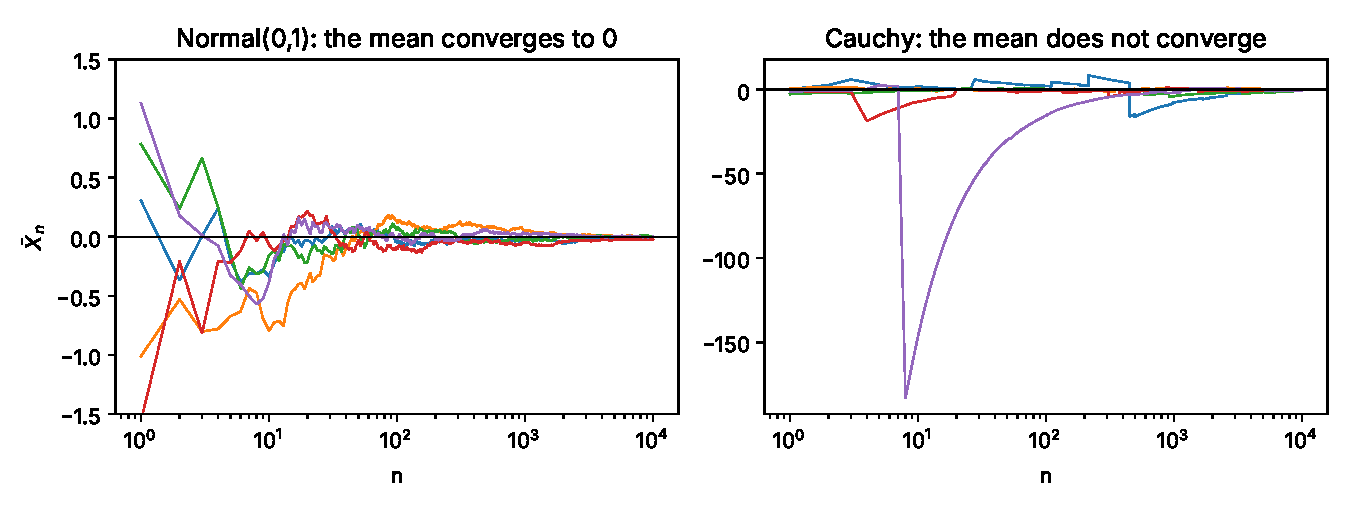
\includegraphics[width=0.95\textwidth]{figures/lln_cauchy.pdf}
\caption{Running sample means along five independent paths. Left: by the SLLN every path converges to $0$. Right: for the Cauchy distribution $\E|X|=\infty$, so occasional huge observations keep making the mean jump.}
\end{figure}

The output shows that the interquartile width of the Cauchy sample mean does \emph{not} shrink at all with $n$; the reason is that $\bar X_n$ is again standard Cauchy (Chapter~\ref{ch:clt}, Example~\ref{ex:cauchy-kf}).

\section{Comments and Notes}

\begin{remark}[The Difference Between the Weak and Strong Laws]
WLLN\index{law of large numbers@law of large numbers!weak wlln@weak (WLLN)}: ``for a fixed large $n$, the probability that $\bar X_n$ is far from $\mu$ is small.'' SLLN\index{law of large numbers@law of large numbers!strong slln@strong (SLLN)}: ``for almost every sequence of observations, the sequence $\bar X_n$ converges to $\mu$.'' Statistical consistency (Chapter~\ref{ch:nokta-tahmin}) is usually defined via the weak version; but the ``one long run'' logic of Monte Carlo\index{monte carlo method@Monte Carlo method} methods relies on the strong version.
\end{remark}

\begin{remark}[The Role of the Assumptions]
The variance condition in the WLLN is for convenience of proof (Khinchin\index{khinchin s theorem@Khinchin's theorem} requires only $\E|X|<\infty$), but the \emph{existence of the mean} is indispensable, as the Cauchy example clearly shows. This is the theoretical reason why, for very heavy-tailed data (financial returns, network traffic), robust estimators such as the median or a trimmed mean are preferred to the sample mean.
\end{remark}

% --- CHAPTER SUMMARY ---
\section{Chapter Summary}
\begin{summary}
\begin{itemize}
  \item Markov's and Chebyshev's inequalities (Theorems~\ref{thm:markov} and~\ref{thm:chebyshev}) bound tail probabilities by moments. The Chernoff and Hoeffding (Theorem~\ref{thm:hoeffding}) bounds give exponentially decaying bounds in return for an MGF or boundedness.
  \item Hierarchy of convergence (Theorem~\ref{thm:hiyerarsi}): almost sure and $L^p$ convergence imply convergence in probability; the converses are false in general.
  \item The weak law of large numbers follows from Chebyshev under a finite variance (Theorem~\ref{thm:wlln}). Khinchin's version requires only $\E|X_1|<\infty$ (Theorem~\ref{thm:khinchin}). The strong law gives almost sure convergence (Theorem~\ref{thm:slln}).
  \item Convergence in probability is preserved under continuous maps (Theorem~\ref{thm:cmt-p}); this is how consistency of estimators carries over to their functions.
  \item In sample-size planning, the Chebyshev and Hoeffding bounds are safe but conservative; the CLT-based rule is approximate.
\end{itemize}
\end{summary}
% --- END OF CHAPTER SUMMARY ---

\paragraph{Further reading.} \cite[Section~5.5]{casella}, \cite[Chapters~4--5]{wasserman}; for measure-theoretic proofs of the laws of large numbers see \cite[Chapter~2]{durrett}.

\section{Exercises}

\begin{exercise}\label{exr:05-1}
Prove the one-sided Chebyshev (Cantelli) inequality: $\P(X-\mu\ge t)\le\frac{\sigma^2}{\sigma^2+t^2}$, $t>0$. (Hint: for every $u\ge0$, $\P(X-\mu\ge t)\le\P((X-\mu+u)^2\ge(t+u)^2)$; apply Markov and then minimise over $u$.)
\hfill\hyperref[coz:05-1]{\footnotesize$\rightarrow$\,Solution}
\end{exercise}

\begin{exercise}\label{exr:05-2}
For $X\sim\text{Poisson}(\lambda)$, compute the Chernoff bound and show that $\P(X\ge a)\le e^{-\lambda}(e\lambda/a)^a$ for $a>\lambda$. Compare Chebyshev, Chernoff and the exact value for $\lambda=10$, $a=20$.
\hfill\hyperref[coz:05-2]{\footnotesize$\rightarrow$\,Solution}
\end{exercise}

\begin{exercise}\label{exr:05-3}
Show, using Borel--Cantelli, that if $X_n\pto X$ then $\{X_n\}$ has a subsequence converging almost surely.
\hfill\hyperref[coz:05-3]{\footnotesize$\rightarrow$\,Solution}
\end{exercise}

\begin{exercise}\label{exr:05-4}
Estimate $\pi$ by Monte Carlo: for $(U_1,U_2)\iid\text{Uniform}(0,1)$, $\P(U_1^2+U_2^2\le1)=\pi/4$. Using Hoeffding's inequality, find the sample size needed to estimate $\pi$ to within $\pm0.01$ with $99\%$ confidence.
\hfill\hyperref[coz:05-4]{\footnotesize$\rightarrow$\,Solution}
\end{exercise}

\chapterlinks{05}

\end{document}
